% =============================================================================
%  fig_pipeline_flowchart.tex
%  Ten-step estimation-adaptation pipeline flowchart
% =============================================================================
\documentclass[tikz, border=6pt]{standalone}
\usepackage{tikz}
\usepackage{amsmath}
\usetikzlibrary{shapes.geometric, shapes.misc, arrows.meta, positioning, calc}

\definecolor{startC}  {RGB}{ 44, 160,  44}
\definecolor{procC}   {RGB}{ 31, 119, 180}
\definecolor{decC}    {RGB}{214,  39,  40}
\definecolor{ioC}     {RGB}{148, 103, 189}
\definecolor{endC}    {RGB}{ 80,  80,  80}

\tikzset{
  start/.style  = {rounded rectangle, draw=startC,  fill=startC!12,  line width=0.9pt,
                   align=center, font=\small, minimum width=3.8cm, minimum height=0.75cm},
  proc/.style   = {rectangle,         draw=procC,   fill=procC!10,   line width=0.8pt,
                   align=center, font=\small, text width=3.5cm,  minimum height=0.85cm},
  proc2/.style  = {rectangle,         draw=ioC,     fill=ioC!10,     line width=0.8pt,
                   align=center, font=\small, text width=3.5cm,  minimum height=0.85cm},
  dec/.style    = {diamond, aspect=2.6, draw=decC,  fill=decC!10,    line width=0.8pt,
                   align=center, font=\small, inner sep=2pt},
  fin/.style    = {rounded rectangle, draw=endC,    fill=endC!12,    line width=0.9pt,
                   align=center, font=\small, minimum width=3.8cm, minimum height=0.75cm},
  arr/.style    = {-{Stealth[length=4.5pt]}, line width=0.85pt, color=gray!70!black},
  lbl/.style    = {font=\scriptsize, color=gray!60!black},
  stepnum/.style = {circle, draw=gray, fill=white, font=\scriptsize\bfseries,
                   inner sep=1.5pt, minimum size=0.45cm},
}

\begin{document}
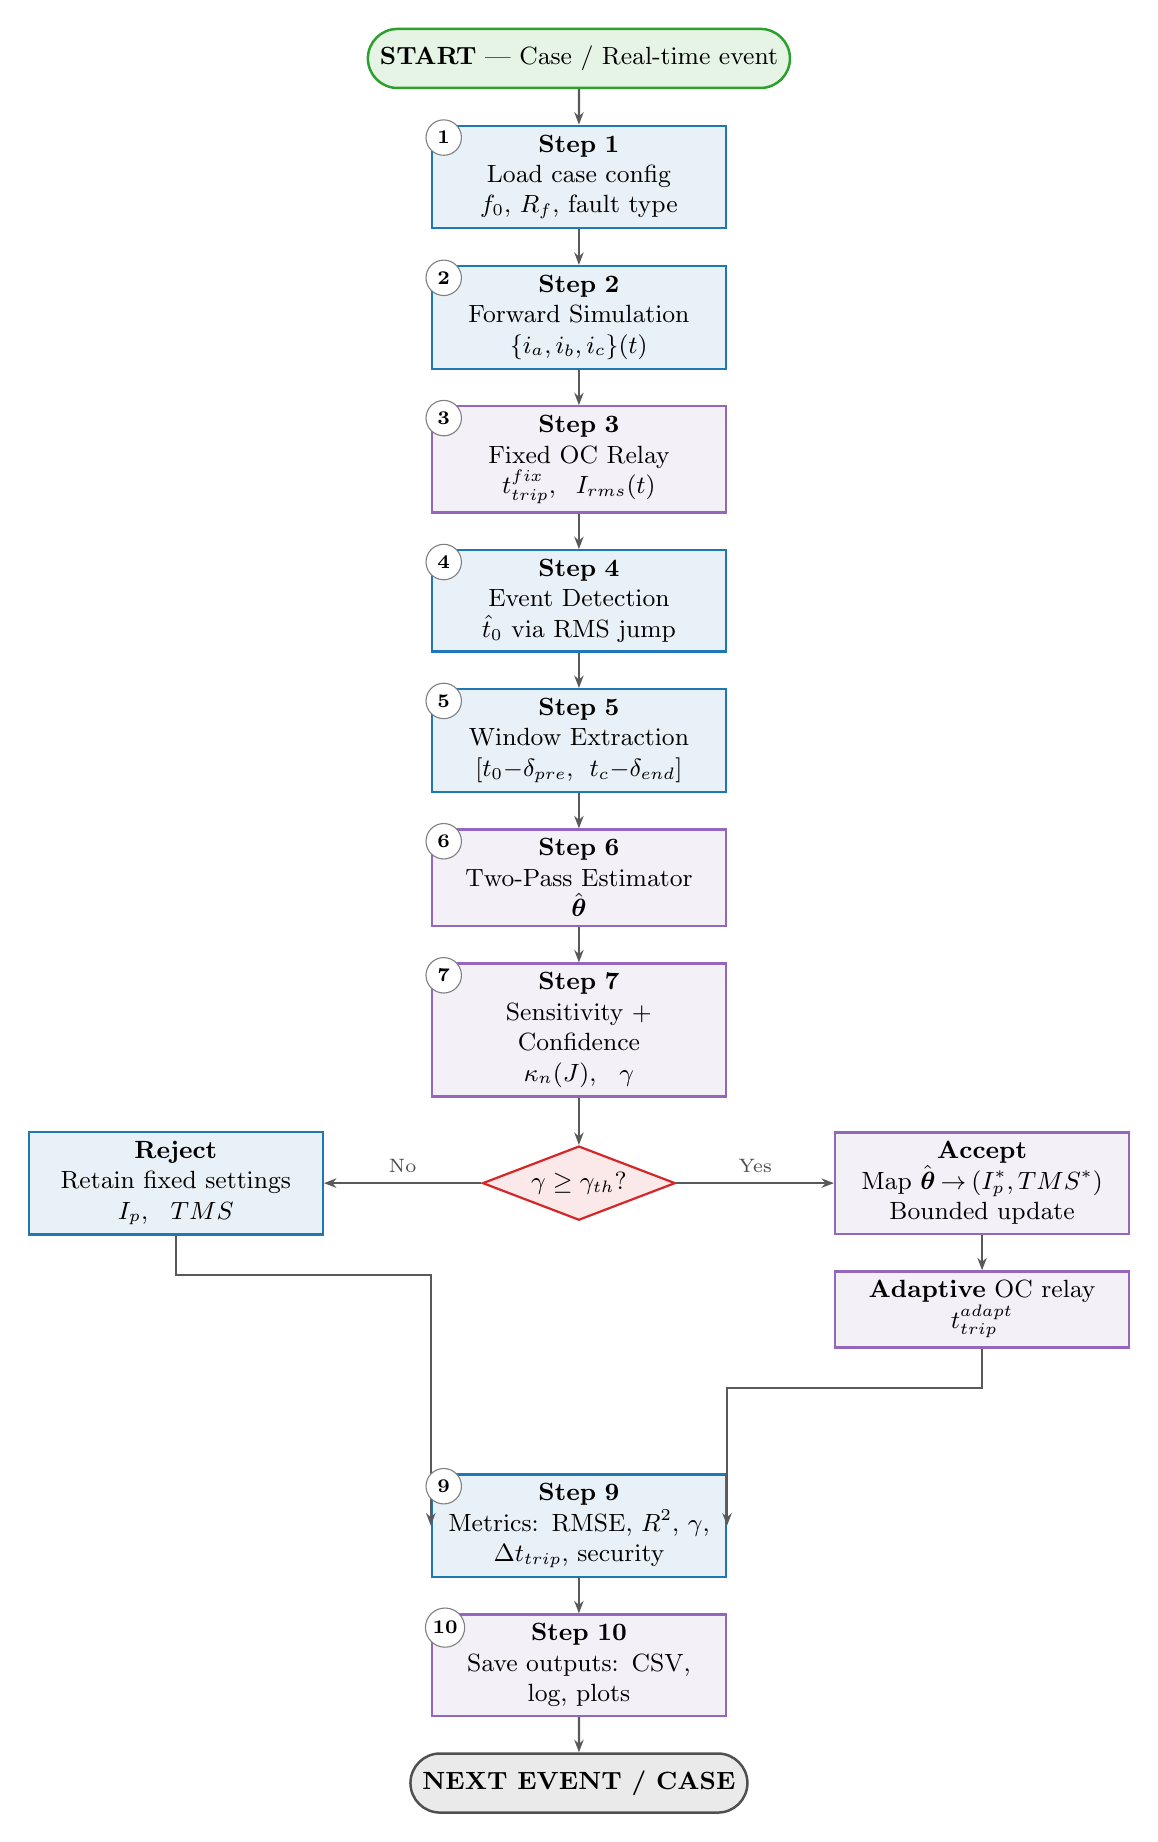
\begin{tikzpicture}[node distance=0.45cm]

% ---- Nodes ------------------------------------------------------------------
\node[start]  (S)   {\textbf{START} — Case / Real-time event};

\node[proc,   below=of S]   (S1)
  {\textbf{Step 1}\\Load case config\\$f_0,\,R_f,\,\text{fault type}$};

\node[proc,   below=of S1]  (S2)
  {\textbf{Step 2}\\Forward Simulation\\ $\{i_a,i_b,i_c\}(t)$};

\node[proc2,  below=of S2]  (S3)
  {\textbf{Step 3}\\Fixed OC Relay\\$t_{trip}^{fix},\;I_{rms}(t)$};

\node[proc,   below=of S3]  (S4)
  {\textbf{Step 4}\\Event Detection\\$\hat{t}_0$ via RMS jump};

\node[proc,   below=of S4]  (S5)
  {\textbf{Step 5}\\Window Extraction\\ $[t_0{-}\delta_{pre},\;t_c{-}\delta_{end}]$};

\node[proc2,  below=of S5]  (S6)
  {\textbf{Step 6}\\Two-Pass Estimator\\ $\hat{\boldsymbol{\theta}}$};

\node[proc2,  below=of S6]  (S7)
  {\textbf{Step 7}\\Sensitivity + Confidence\\ $\kappa_n(J),\;\gamma$};

\node[dec,    below=0.6cm of S7] (D1)
  {$\gamma \geq \gamma_{th}$?};

% ---- Right branch (accept) — flows downward from diamond -------------------
\node[proc2,  right=2.0cm of D1] (S8a)
  {\textbf{Accept}\\Map $\hat{\boldsymbol{\theta}}\!\to\!(I_p^*,TMS^*)$\\Bounded update};

\node[proc2,  below=0.45cm of S8a] (S8b)
  {\textbf{Adaptive} OC relay\\$t_{trip}^{adapt}$};

% ---- Left branch (reject) ---------------------------------------------------
\node[proc,   left=2.0cm of D1]  (S8c)
  {\textbf{Reject}\\Retain fixed settings\\$I_p,\;TMS$};

% ---- Step 9/10 below decision row -------------------------------------------
\node[proc,   below=3.2cm of D1] (S9)
  {\textbf{Step 9}\\Metrics: RMSE, $R^2$, $\gamma$,\\$\Delta t_{trip}$, security};

\node[proc2,  below=of S9]  (S10)
  {\textbf{Step 10}\\Save outputs: CSV,\\log, plots};

\node[fin,    below=of S10] (E)  {\textbf{NEXT EVENT / CASE}};

% ---- Arrows: main spine -----------------------------------------------------
\draw[arr] (S)  -- (S1);
\draw[arr] (S1) -- (S2);
\draw[arr] (S2) -- (S3);
\draw[arr] (S3) -- (S4);
\draw[arr] (S4) -- (S5);
\draw[arr] (S5) -- (S6);
\draw[arr] (S6) -- (S7);
\draw[arr] (S7) -- (D1);

% ---- Decision branches ------------------------------------------------------
\draw[arr] (D1.east) -- node[lbl, above]{Yes} (S8a.west);
\draw[arr] (D1.west) -- node[lbl, above]{No}  (S8c.east);
\draw[arr] (S8a)     -- (S8b);

% ---- Merge to Step 9 — clean right-angle paths ------------------------------
\draw[arr] (S8b.south) -- ++(0,-0.5) -| (S9.east);
\draw[arr] (S8c.south) -- ++(0,-0.5) -| (S9.west);

\draw[arr] (S9)  -- (S10);
\draw[arr] (S10) -- (E);

% ---- Step number badges -----------------------------------------------------
\foreach \nd/\num in {S1/1, S2/2, S3/3, S4/4, S5/5, S6/6, S7/7, S9/9, S10/10}
  \node[stepnum, anchor=north west] at (\nd.north west) {\num};

\end{tikzpicture}
\end{document}
